% ===============================
% Slide: Tổng quan Python Server
% ===============================

\begin{frame}[fragile]{Python Server: Kiến trúc & Luồng Xử lý}
\small
\begin{columns}[T, totalwidth=\textwidth]

    % ---------------- Column 1: Kiến trúc + Quy trình ---------------- %
% --- Cột text: Kiến trúc & Quy trình ---
    \begin{column}{0.48\textwidth}
        % --- Kiến trúc phân tầng ---
        \begin{block}{Kiến trúc phân tầng}
            \scriptsize
            \textbf{Thu nhận:} \texttt{comm/} (MQTT, Telegram, AMI), \texttt{detection/} (video, tracking)\\[0.2em]
            \textbf{Xử lý:} \texttt{fall/}, \texttt{processing/}\\[0.2em]
            \textbf{Đầu ra:} \texttt{database/}, cảnh báo
        \end{block}

        % --- Luồng xử lý ---
        \begin{block}{Luồng Xử lý}
            \scriptsize
            1. Thu nhận: ESP32 (MQTT), Camera IP (AI)\\
            2. Tích hợp: \texttt{DetectionProcessor} đồng bộ dữ liệu\\
            3. Đầu ra: Lưu sự kiện, gửi cảnh báo qua AMI/Telegram
        \end{block}
    \end{column}
    % ---------------- Column 2: Hình minh họa ---------------- %
    \begin{column}{0.52\textwidth}
        \begin{figure}
            \centering
            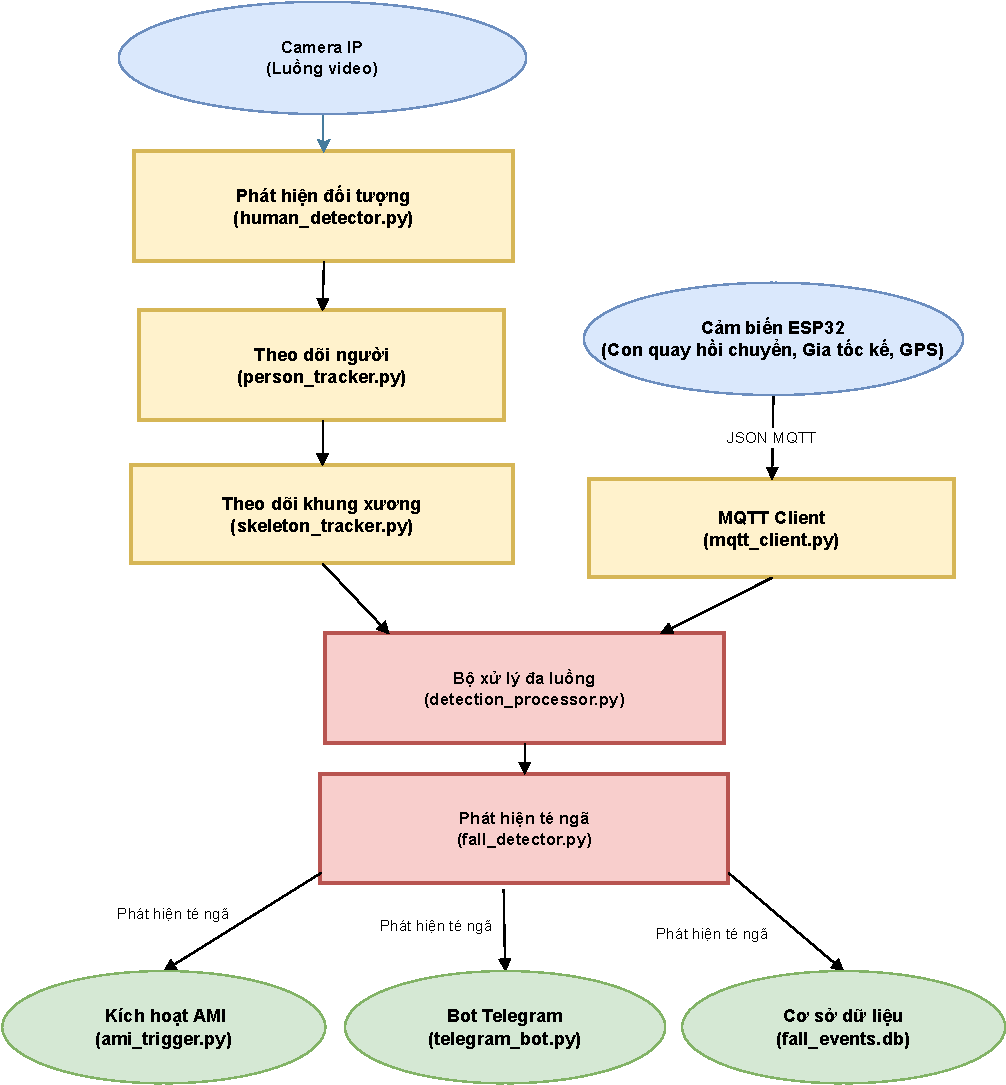
\includegraphics[width=\linewidth,height=0.80\textheight,keepaspectratio]{images/server_flow.pdf}
            \caption{\footnotesize Luồng dữ liệu qua \texttt{DetectionProcessor}}
        \end{figure}
    \end{column}

\end{columns}
\normalsize
\end{frame}
% ===============================
% Slide: Thuật toán phát hiện té ngã
% ===============================

\begin{frame}[fragile]{Python Server: Thuật toán Phát hiện Té ngã}
\scriptsize
\begin{columns}[T,onlytextwidth]
    % --- Cột 1: Thuật toán ---
    \begin{column}{0.48\textwidth}
        \begin{block}{Quy trình trong \texttt{FallDetector}}
            \textbf{Kiểm tra:} Landmarks hợp lệ (độ tin cậy $\geq 0.5$)\\[0.2em]
            \textbf{Tính toán:} Góc thân ($>60^\circ$ dọc, $>45^\circ$ ngang), vận tốc thân ($>0.5$ đơn vị)\\[0.2em]
            \textbf{Trạng thái:} \textit{Falling} nếu góc + vận tốc vượt ngưỡng, \textit{Lying} nếu góc vượt ngưỡng kéo dài\\[0.2em]
            \textbf{Quyết định:} Bộ đếm $\geq 5$ frame → té ngã, reset trạng thái
        \end{block}
    \end{column}

    % --- Cột 2: Hình minh họa ---
    \begin{column}{0.5\textwidth}
        \begin{figure}
            \centering
            \includegraphics[width=\linewidth,height=0.8\textheight,keepaspectratio]{images/python_fall_diagram.pdf}
            \caption{Luồng thuật toán phát hiện té ngã}
            \label{fig:python_fall_diagram}
        \end{figure}
    \end{column}
\end{columns}
\end{frame}
